\section{Dynamical activation}\label{sec:activation}
\Cref{thm:A4T1} exhibits a pair $(x,y)$ in which relations dormant at $x$ are realised at $y$. The dynamical question is whether $y$ lies on the collective orbit of $x$. This section proves the structure of $\Kmove(y)$, the necessary conditions, an obstruction, and a closed form for the arrival of the activating occurrences, and then presents the complete eight-step and $375$-step trajectories as exact finite examples. Throughout, the family data of \cref{thm:A4T1} are fixed; write $N=P-1=\ell m$.

\subsection{The geometry of the activated state}
\begin{theorem}[the move complex of the activated state]\label{thm:A4T2}
In the setting of \cref{thm:A4T1}, $\Kmove(y)$ is the complete graph $K_{k+1}$ on the vertices $P,p_1q,\dots,p_kq$ with no $2$-cells; hence $\beta_1(\Kmove(y))=k(k-1)/2$ and $\beta_i=0$ for $i\ge2$. $\Kaxis(y)$ is a discrete set of $k+1$ points, and $\Kmove(x)$ is a point. For $k=2$ this is a triangle with $\beta_1=1$. Moreover $|\Gr(y)|=(k+1)(k+2)$ for $k=2,\dots,5$ (\stat{finite-exact}).
\end{theorem}
\prov{CW-0424}{A4-T2}{MIXED}{SPLIT}
\begin{proof}
The fibre of $y$ is $\{P,p_1q,\dots,p_kq\}$ with exponent vectors $\mathbf 1=\sum_je_j$ and $e_i+e_q$. The vectors $e_i-e_j$ ($i\ne j$) are edges, as shown in the proof of \cref{thm:A4T1}; they join all pairs of the $k$ vertices $p_iq$. The vertex $P$ and $p_iq$ differ by $g=\sum_{j\ne i}e_j-e_q$; the coordinate hull $H(P,p_iq)$ consists of points whose $p_i$-coordinate is $1$, so it excludes the origin, and by the classification of fibre points it contains no fibre point other than the endpoints; by \cref{lem:hull}, $g\in\Gr(y)$ and $\{P,p_iq\}$ is an edge. So the $1$-skeleton is $K_{k+1}$. A $2$-cell would be a parallelogram $w_1,w_2,w_3,w_4$ of distinct fibre points with $w_1+w_4=w_2+w_3$. The $q$-coordinate is $0$ for $P$ and $1$ for each $p_iq$. If $P$ is not among the four, the relation reads $e_a+e_b=e_c+e_d$ on the $p$-coordinates with $\{a,b\}=\{c,d\}$, contradicting distinctness; if $P$ is among them, the two sides have $q$-coordinate sums $0+1$ and $1+1$ (or $0+0$ against $2$), which differ. Hence there are no $2$-cells and $\beta_1=\binom{k+1}2-k=\binom k2$ for the connected graph. $\Kaxis(y)$: two fibre points differ by a unit vector $\pm e_p$ never (their differences are of the above types), so there are no axis edges. $\Kmove(x)$ is the single fibre point $\mathbf 1$. The value $|\Gr(y)|=(k+1)(k+2)$ was found by exhaustive enumeration with the independent engine (Appendix~\ref{app:relations}). \qedhere
\end{proof}
The activation family for $k=2$ is drawn in \cref{fig:family}, and the complete graphs for larger $k$ in \cref{fig:completegraph}.
\begin{figure}[tbp]\centering
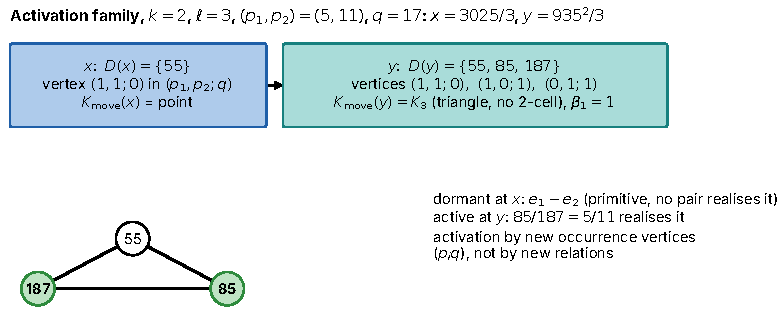
\includegraphics[width=\textwidth]{fig13_activation_family}
\caption{\textbf{The activation family, $k=2$ (exact; proved by \cref{thm:A4T1,thm:A4T2}).} Parameters: $\ell=3$, $(p_1,p_2)=(5,11)$, $q=17$, $x=3025/3$, $y=935^2/3$. Left box: $x$ has a single occurrence vertex, $55$. Right box: $y$ has $D(y)=\{55,85,187\}$ and its move complex is the triangle $K_3$ with no $2$-cell, $\beta_1=1$. The relation $e_1-e_2$ is primitive but realised by no pair at $x$ (dormant) and realised by $85/187=5/11$ at $y$: activation by new occurrence vertices, not creation of a relation. The abstract objects are the Graver vectors; the geometric object is the complex.}\label{fig:family}
\end{figure}
\begin{figure}[tbp]\centering
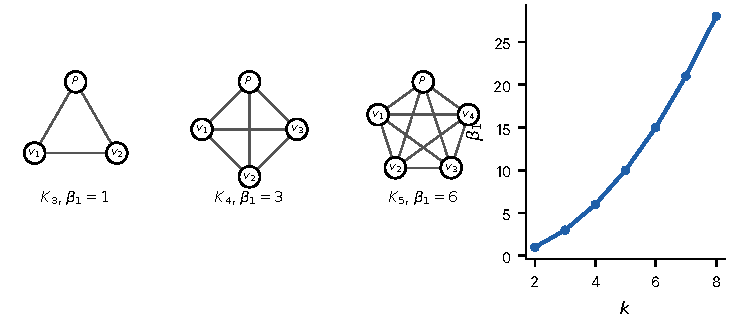
\includegraphics[width=\textwidth]{fig14_complete_graph}
\caption{\textbf{The complete graph $K_{k+1}$ (exact; proved by \cref{thm:A4T2}).} $k=2,3,4$: the move complex of $y$ with vertices $P,v_i=p_iq$ (abstract layout; not a geometric embedding), $\beta_1=1,3,6$. Right: $\beta_1=k(k-1)/2$ for $k=2,\dots,8$ is the proved formula; the values $k=2..5$ were recomputed by the engine and $k\ge6$ are formula values (labelled as such), not computations.}\label{fig:completegraph}
\end{figure}

\subsection{Progression, necessary conditions, blocking}
\begin{lemma}[progression]\label{lem:progression}
From $x=P^2/\ell$ the orbit is $x_j=P^2(m+j)/(\ell m)=P^2u/N$, $u=m+j$, as long as $D(x_j)=\{P\}$, and $P\in D(x_j)$ always. The first state with $D\ne\{P\}$ lies on this line. The line reaches $y$ exactly at $u=q^2m$.
\end{lemma}
\begin{proof}
$D(x)=\{P\}$, $L=P$, $G=P-1=N$ (as $G$ divides $N$ and $P-1\in\{d-1\}$), $b=\ell$, $h=m$, $Y_j=P^2(m+j)$. For $d=P$: $r(P)=1$ and $Q(P)=P^2$ (as $v_p(N)=0$ for $p\mid P$), so $P\in D$ by \cref{thm:sieve}. The state with $u=q^2m$ equals $P^2q^2/\ell=y$. \qedhere
\end{proof}
\begin{theorem}[necessary conditions and blocking criterion]\label{thm:A4T3b}
Suppose $y$ lies on the collective orbit of $x$. Then:
\begin{enumerate}[label=(\arabic*),itemsep=1pt]
\item every state $z$ of the orbit before $y$ satisfies $D(z)\subseteq D(y)=\{P\}\cup\{p_iq\}$;
\item at the first event, at progression index $u$, the new elements are among the $p_iq$, so $q^2\mid u/\gcd(u,N)$ and $p_iq\equiv1\pmod{b_u}$ with $b_u=N/\gcd(u,N)$;
\item the line cannot run to $u=N$: there the state is the integer $P^2$, with $p_i\in D(P^2)\setminus D(y)$.
\end{enumerate}
Conversely, \emph{any} state of an orbit with $D\not\subseteq D(y)$ blocks $y$ forever (blocking criterion).
\end{theorem}
\prov{CW-0426}{A4-T3b}{PROVED}{FULL}
\begin{proof}
(1) and the converse are \cref{lem:M}: $D$ is non-decreasing along the orbit, so a state containing an element outside $D(y)$ is followed only by such states. (2) On the line, the state $P^2u/N$ has reduced denominator $b_u=N/\gcd(u,N)$ and numerator $P^2u/\gcd(u,N)$; $d=p_iq\in D$ requires $q^2\mid u/\gcd(u,N)$ (as $q\nmid P$) and $d\equiv1\pmod{b_u}$. (3) At $u=N$ the state is $P^2\cdot N/N=P^2$; $p_i^2\mid P^2$ so $p_i\in D(P^2)$ (the denominator is $1$), whereas $p_i\notin D(y)=\{P\}\cup\{p_jq\}$ by \cref{thm:A4T1}. \qedhere
\end{proof}

\begin{theorem}[proper-divisor obstruction]\label{thm:A5T11}
For a proper divisor $1<d_0<P$, while $D=\{P\}$ one has $d_0\in D(x_u)\iff r(d_0)\mid u$, $r(d_0)=N/\gcd(d_0-1,N)$. Put $u_f=\min_{d_0}(\text{least multiple of }r(d_0)\text{ exceeding }m)$ and $u_a=\min_iu_i$ where $u_i$ is the arrival index of $p_iq$ of \cref{thm:A5T24}. If $u_f\le u_a$ and $u_f<q^2m$, then $y$ is not on the orbit of $x$ (\stat{blocked}).
\end{theorem}
\prov{CW-0453}{A5-T1.1}{PROVED}{FULL}
\begin{proof}
$P$ is squarefree and $p\mid d_0$ implies $p\nmid N$, so $Q(d_0)=\lcm(r(d_0),\prod_{p\mid d_0}p^2)$ and $Q(d_0)\mid P^2u$ iff $r(d_0)\mid u$ ($\gcd(r(d_0),P)=1$ since $r\mid N$). By \cref{thm:sieve} this is the stated equivalence. A proper divisor $d_0$ of the squarefree $P$ is not in $D(y)=\{P\}\cup\{p_iq\}$. Consider the orbit for $u<u_f$. If an event occurs at $u<u_f$, it cannot add only elements of the form $p_iq$ (those arrive at $u\ge u_a\ge u_f$), so some state has $D\not\subseteq D(y)$. If no event occurs before $u_f$, at $u=u_f$ some $d_0$ joins, with the same conclusion; and $y$ (at $u=q^2m>u_f$) was not hit meanwhile, since $D(x_u)=\{P\}\ne D(y)$ for $u<u_f$. In both cases the blocking criterion of \cref{thm:A4T3b} applies. \qedhere
\end{proof}
\begin{theorem}[arrival of the activating occurrences]\label{thm:A5T24}
While $D=\{P\}$, the occurrence $p_iq$ belongs to $D(x_u)$ iff $M_i\mid u$, where $M_i=\lcm\big(r_i,\ q^{2+v_q(N)}\big)$ and $r_i=N/\gcd(p_iq-1,N)$. The earliest arrival is at $u_i=$ the least multiple of $M_i$ exceeding $m$.
\end{theorem}
\prov{CW-0440}{A5-T2.4}{PROVED}{FULL}
\begin{proof}
Apply \cref{thm:sieve} to $d=p_iq$ with $Y=P^2u$, $G=N$: for $p=p_i$ we have $v_{p}(N)=0$ and $p^2\mid P^2$; the prime $q$ has $q\nmid P$ so $q^{2+v_q(N)}\mid P^2u$ iff $q^{2+v_q(N)}\mid u$; and $r_i\mid N$ is coprime to $P$, so $r_i\mid P^2u$ iff $r_i\mid u$. Finally $M_i\nmid m$ because $p_iq\notin D(x)$. \qedhere
\end{proof}
\begin{remark}[finite-exact check]
The closed form was compared with the sieve evaluated directly in $14$ instances: all agree (\stat{finite-exact}). The set $\{M_i\}$ is the object behind the observed phenomenon that the numerical multiplier $q^2$ is \emph{not} the mechanism of arrival: the orbit leaves the line at the first event, and arrives at $y$ by a later exact landing (examples below).
\end{remark}
\begin{counter}[``$q^2>\ell\Rightarrow$ unreachable'']\label{cx:q2l}
The initial conjecture that $q^2>\ell$ forbids reaching $y$ is false: $\ell=3$, $q=2$ has $q^2=4>3$ and $y=110^2/3$ is reached from $x=55^2/3$ in eight steps (\cref{sec:activation}, below).
\end{counter}
\prov{CW-0429}{A4-T3e}{COUNTEREXAMPLE}{EXAMPLE}

\subsection{The eight-step trajectory \texorpdfstring{$3025/3\to12100/3$}{3025/3->12100/3}}
The pair $x=55^2/3=3025/3$, $y=110^2/3=12100/3$ is the member $k=2$, $\ell=3$, $c=2$, $(p_1,p_2)=(5,11)$, $q=2$ of the family ($q=2$, not $17$). Here $P=55$, $N=54$, $m=18$.
\begin{theorem}[$x\to y$ in eight steps]\label{thm:A4T3c}
The collective orbit of $3025/3$ passes through $12100/3$ at step $8$. The denominators are $3,54,27,18,27,54,9,9,3$. The occurrence inventories, move complexes and Betti vectors are those of \cref{tab:t8}: $D=\{55\}$ for $n\le5$ (a point); one event at step $6$ ($D=\{10,55\}$, one edge, a path) and one event at step $8$ ($D=\{10,22,55\}$, a triangle with no $2$-cell). Hence $\beta_1$ passes from $0$ to $1$, at step $8$, and $y$ is reached by activation of $e_{11}-e_5$.
\end{theorem}
\prov{CW-0427}{A4-T3c}{FINITE-EXACT}{FINITE}
\begin{proof}[Exact computation]
Direct iteration of $C$ in rational arithmetic with the independent engine. The first event is predicted by \cref{cor:event,thm:A5T24}: $d=10=5\cdot2$ has $r(10)=54/\gcd(9,54)=6$, $q^{2+v_2(54)}=2^3$, $M=24$, so it arrives at $u=24$, i.e.\ at step $24-18=6$; at this step $L=110$ and $G=9$ change, and the second stage ($D=\{10,55\}$, $b=9$) lands on $y$ two steps later, with the new element $22$. \qedhere
\end{proof}
\begin{table}[tbp]\centering\small
\begin{tabular}{@{}rrrlrl@{}}\toprule
$n$ & $x_n$ & $b_n$ & $D(x_n)$ & move edges & $(\beta_0,\beta_1)$\\\midrule
0 & $3025/3$ & 3 & $\{55\}$ & 0 & $(1)$\\
1 & $57475/54$ & 54 & $\{55\}$ & 0 & $(1)$\\
2 & $30250/27$ & 27 & $\{55\}$ & 0 & $(1)$\\
3 & $21175/18$ & 18 & $\{55\}$ & 0 & $(1)$\\
4 & $33275/27$ & 27 & $\{55\}$ & 0 & $(1)$\\
5 & $69575/54$ & 54 & $\{55\}$ & 0 & $(1)$\\
6 & $12100/9$ & 9 & $\{10,55\}$ & 1 & $(1)$\\
7 & $24200/9$ & 9 & $\{10,55\}$ & 1 & $(1)$\\
8 & $12100/3$ & 3 & $\{10,22,55\}$ & 3 & $(1,1)$\\
\bottomrule\end{tabular}
\caption{\textbf{The eight-step orbit $x_0=3025/3$} (exact, \cref{thm:A4T3c}). Events occur at $n=6$ (new occurrence $10$) and $n=8$ (new occurrence $22$); the move complex of $D$ gains the edge $\{10,55\}$ at $n=6$ and the triangle with edges $\{10,22\},\{10,55\},\{22,55\}$ at $n=8$, so $\beta_1$ rises $0\to1$ at the last step only. The state $x_8=12100/3=(55\cdot2)^2/3$ is the activated target with $q=2$.}\label{tab:t8}
\end{table}

\begin{remark}[$q=2$ versus $q=17$; blocking]
For the same $x$ and $q=17$ the target $y'=935^2/3$ is blocked (\cref{thm:A5T11}: $u_f=27\le u_a=2601$ and $u_f<q^2m$; concretely the first event at step $6$ adds $10\notin D(y')$). Reachability depends on $q$, not on $q^2>\ell$ (\cref{cx:q2l}).
\end{remark}
\Cref{fig:eight} plots the eight-step trajectory of \cref{tab:t8}.
\begin{figure}[tbp]\centering
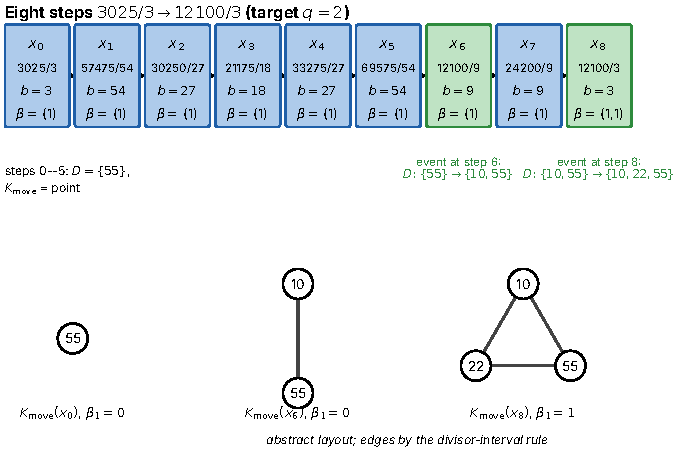
\includegraphics[width=\textwidth]{fig15_eight_step}
\caption{\textbf{The eight-step trajectory (finite-exact; exact computation).} $x_0=3025/3$, $n=0..8$, $\ell=3$, $q=2$. Each box gives $x_n$, its denominator $b_n$ and the Betti vector of $\Kmove(x_n)$ (boxes shaded green at the two event steps $6$ and $8$). Below: the move complexes at steps $0$, $6$, $8$ (abstract layout; edges by the divisor-interval rule of \cref{sec:interval}); $D$ changes only at the two events, the topology changes only at the second.}\label{fig:eight}
\end{figure}

\subsection{The \texorpdfstring{$375$}{375}-step three-prime example}
\begin{theorem}[$k=3$, $\ell=7$: $x\to y$ in $375$ steps]\label{thm:A4T3c375}
Let $(p_1,p_2,p_3)=(11,53,67)$, $P=39061$, $q=2$, $\ell=7$, $x=P^2/7$, $y=(2P)^2/7$. The orbit of $x$ reaches $y$ at step $375$. The events are at steps $372$ (new element $106=2\cdot53$), $373$ ($22=2\cdot11$) and $375$ ($134=2\cdot67$), and $\beta_1(\Kmove)$ is $0$ up to step $372$, $0$ after it, $1$ after step $373$ and $3$ after step $375$. The progression of \cref{lem:progression} alone would need $q^2m-m=16740$ steps.
\end{theorem}
\prov{CW-0427}{A4-T3c}{FINITE-EXACT}{FINITE}
This is an \emph{exact finite example}: it is computed, step by step, with the independent engine; it is not a general reachability result. The complex after the last event is $K_4$ ($P$ and the three $p_iq$, with $|D|=4$ and six edges), so $\beta_1=3$ agrees with \cref{thm:A4T2}. \Cref{fig:375} shows the denominators and the last twelve steps.
\begin{figure}[tbp]\centering
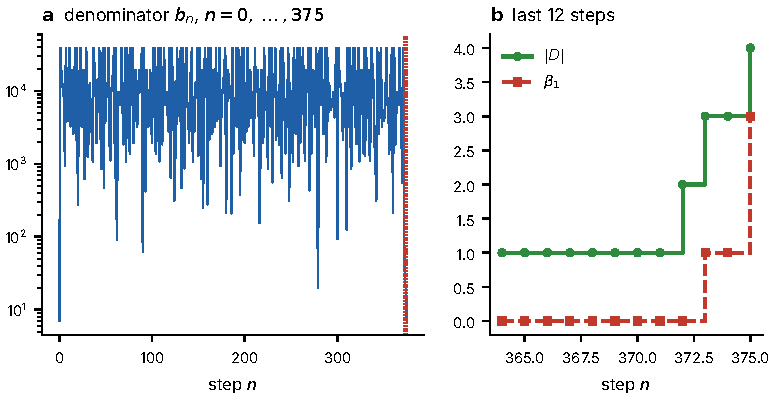
\includegraphics[width=\textwidth]{fig16_375_step}
\caption{\textbf{The $375$-step orbit (finite-exact; exact computation).} $x_0=39061^2/7$, $n=0..375$. (a) Reduced denominator $b_n$ (log scale); dotted lines mark the events at $n=372,373,375$. (b) Last twelve steps: $|D(x_n)|$ and $\beta_1$ of $\Kmove(x_n)$; $\beta_1$ is $0$ up to $n=372$, $1$ for $n=373,374$ and $3$ at $n=375$.}\label{fig:375}
\end{figure}

\subsection{Reachability scope}
The decision problem (is $y$ on the orbit of $x$?) is settled by an exact stage-jumping decider: follow the orbit stage by stage with the sieve; inside a stage landing on $y$ is an integrality condition on $(y-x_j)L^{-2}G$, and \cref{lem:M} supplies the blocking test. It is exact but not known to terminate on every input.
\begin{proposition}[cited finite data on reachability]\label{prop:reach}
The following are \stat{cited} from the source release (A4-T3c table, A5-T1.2, A5-T1.3), not re-run here:
(i) among $993$ pairs ($\ell=3$ with $q\in\{2,5,11,17,23,29\}$; $\ell=5,7$ with $k=2$; $\ell=7$, $k=3$, $q=2$), $40$ are reached, $929$ blocked, $24$ were unresolved at the step cap and none overshot; the $24$ were later decided exactly: $22$ blocked and $2$ reached (for $k=3$, $\ell=7$, $q=2$, $(67,151,179)$ in $45{,}666$ steps and $(151,179,193)$ in $67{,}756$ steps);
(ii) in a scan of $k=2$ pairs ($p<2000$, $P\le300{,}000$, $q<90$), $\ell=3$ has $52{,}997$ pairs of which $1{,}131$ are reached, $\ell=5$ has $4{,}010$ pairs of which one is reached, and the reached $q$ include $11,17$ ($\ell=3$) and $19$ ($\ell=5$: $(89,1709)$ in $2{,}239$ steps). The statement ``reached members occur only for $q\in\{2,5\}$'' is therefore false and is not repeated.
\end{proposition}
\prov{CW-0454}{A5-T1.2}{FINITE-EXACT}{CITED}
\prov{CW-0455}{A5-T1.3}{FINITE-EXACT}{CITED}
The cases re-examined here are exact: $(5,11)$, $q=2$ reached in $8$ steps; $(5,11)$, $q=17$ blocked at the first event (adds $10$); $(29,647)$, $\ell=3$, $q=11$ reached in $938$ steps; $(47,1613)$, $q=17$ in $2318$ steps; $(89,1709)$, $\ell=5$, $q=19$ in $2239$ steps; $(11,53,67)$, $\ell=7$, $q=2$ in $375$ steps (\stat{finite-exact}).
\begin{problem}[A4-T3f: infinite reached subfamily; no overshoot; closed form of the arrival step]\label{prob:A4T3f}
Is the set of reached members infinite? Is every non-blocked member reached (no overshoot; none seen among the resolved rows)? Is there a closed form for the step at which an orbit lands on $y$? \Cref{thm:A5T24} gives only the first arrival of an activating occurrence along the progression.
\end{problem}
\prov{CW-0430}{A4-T3f}{OPEN}{OPEN}

\subsection{Activation at step level, and activation without a change of Betti numbers}
\begin{proposition}[step-level activation without excursion]\label{prop:A4T3d}
(i) On the orbit of $126^2/5$ (the $G=5$ tower of \cref{thm:R3T5c}, $k=0$), at the step $5\to6$ (tower index $1\to2$) the set $D=\{6,21,36,126\}$ gains $56$, the number of dormant primitive relations drops from $6$ to $0$ and $\beta_1$ of $\Kmove$ passes from $1$ to $4$. (ii) For $\ell=29$, $x_0=1890^2/29$, at step $23\to24$ $D$ gains $175$, the number of dormant relations drops from $4$ to $2$ and the Betti vector passes from $(1)$ to $(1,1)$. (\stat{finite-exact}.)
\end{proposition}
\prov{CW-0428}{A4-T3d}{FINITE-EXACT}{FINITE}
\begin{proposition}[activation need not change Betti numbers]\label{prop:A4T4c}
There are activation events with $\beta(\Kmove)$ unchanged: the first is $\ell=5$, $S=36$, $x_0=S^2/5$, step $3\to4$, with Betti vector $(1)\to(1)$. Among the $474$ step-activation events of the source census ($\ell=5,7,11,13$; $382$ orbits), $394$ change the Betti vector, $80$ do not, and $57$ lower $\beta_1$ (\stat{cited}). In the recomputed census of all $2{,}576$ occurrence events of the orbits $x_0=S^2/\ell$ ($L=S$, $G=\ell$, $S<1500$, $24$ steps; \cref{thm:A5T7}), a different sample from the source's $474$ events,, $1{,}787$ leave the Betti vector unchanged, $603$ raise it, $172$ lower it and $14$ both raise and lower (\cref{sec:homology}). Thus the implication ``activation $\Rightarrow$ topology change'' is false in general, and it is also false that activation always raises homology.
\end{proposition}
\prov{CW-0433}{A4-T4c}{COUNTEREXAMPLE}{CITED}
\Cref{fig:unchanged} records an event with unchanged Betti numbers.
\begin{figure}[tbp]\centering
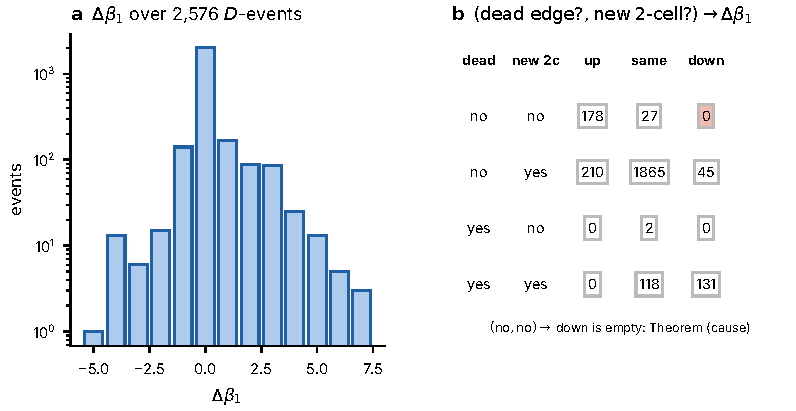
\includegraphics[width=\textwidth]{fig17_unchanged_betti}
\caption{\textbf{Occurrence events do not determine the sign of the homology change (finite-exact; $2{,}576$ events, $382$ orbits, $\ell=5,7,11,13$).} (a) Distribution of $\Delta\beta_1$ (log scale). (b) Counts by mechanism: whether the event kills an old edge (``dead'') and whether it creates a $2$-cell (``new $2$c''), against the sign of $\Delta\beta_1$. The cell (no dead edge, no new $2$-cell) with $\Delta\beta_1<0$ is empty, as proved in \cref{thm:zigzag}. Checked range only; the census is a finite sample, not a statement about all orbits.}\label{fig:unchanged}
\end{figure}
